\documentclass{llncs}
\pagestyle{headings}
\usepackage[utf8]{inputenc}
\usepackage[
backend=biber,
style=alphabetic,
sorting=ynt
]{biblatex}
\addbibresource{sample.bib}
\usepackage{graphicx}


\begin{document}

\title{%
Mobile machine learning}

\author{%
Ruben Teimas}
\authorrunning{R. Teimas}

\institute{%
  Universidade de Évora, Portugal\\
  \email{m47753@alunos.uevora.pt}
 }

\date{}


\maketitle{}

\begin{abstract}
This papers starts by briefly presenting the history of mobile technology and machine learning, giving context of how we got to where here are. It then investigates the advantages of coupling these technologies and why that cooperation has been so impactful for the world and gives a brief perspetive of the future of computer interaction.
\keywords{Mobile Computing \and machine learning \and Internet of Things \and Data Collection}
\end{abstract}


\section{Introduction}

Mobile computing was one of the hottest trends at the turn of the century with the appearance of \emph{PDA}s but it wasn't until around mid 2000 that the users massively engaged with this type of technology, when \emph{Apple} launched the first \emph{iPhone} and the first \emph{Smartphones} came up.\\

Since then mobile computing has come a long way, being the primary way of interaction with technology, leaving the desktops and other traditional forms of interaction behind, mostly used in specific tasks.\\

Another hot trend at the beginning of 2010's was \emph{Artificial Intelligence}, more specifically \emph{machine learning} and \emph{Deep Learning}. Nowadays most of the companies use it, or at least they claim to. 

It has enabled us to make predictions, to interact with technology in non-conventional ways (voice and video), create \emph{smart cities} and tailored customer experiences.\\

Inevitably this two technologies have been  working side-by-side and pushing us further as a society, making information more accessible, creating new experiences and improving existing ones.

\section{Mobile Devices}
\subsection{What are mobile devices?}
There's not an exact definition for a mobile device, these however usually share some characteristics: touchscreen interfaces with color display, rechargeable batteries and can connect over wireless networks.\\

Over time some devices that were once considered mobile devices are no longer considered. One of those examples is the \emph{Tablet}. When it appeared it was considered a mobile device since it had the characteristics described above, nonetheless many people do not considered it a mobile device claiming it has more similarities with a laptop than with a smartphone specially due to its size.\\

Today's most popular mobile devices are smartphones and smartwatches.
\subsection{The rise of mobile devices}
When \emph{Apple} presented the first \emph{iPhone}, in 2007, it changed the world's perception of what a phone could, and should, be.\\

\emph{iPhone} did not only improved existing features that other phones had at the time, like call making, texting, music and video reproduction as it introduced new (almost) features, such as totally functional touchscreen that allowed the user to control the phone without using (physical) buttons, a satisfiable way to browse the web, the concept of \emph{mobile apps} that could be installed trough the \emph{App Store}, light and proximity sensors, accelerometer and many more!\\

Around the same time there was a project in development, that had been acquired by \emph{Google}: the \emph{Android}.

The \emph{Android} operating system was based on the \emph{Linux} kernel that would power "intelligent" mobile devices which would be more aware of user's preferences and location.\\

Even though \emph{Apple} and \emph{Google} had different visions and philosophy both their technology pushed the mobile computing further.

A survey \cite{mobile_usage} concluded that, in 2020, 68\% of the web visits, globally, were made by mobile devices (not considering \emph{Tablets} as mobile devices).\\


\section{machine learning}
\subsection{Artificial Intelligence and machine learning}
Being amongst the most trendy technologies of 2021 \cite{trend_tech} these words almost always appear together which sometimes misleads people to think they are the same.\\

Artificial Intelligence (\emph{AI}) is the a broad concept which defines every system that can simulate the human intelligence.

By narrowing the concept of \emph{AI} new concepts came up, one of them was machine learning (\emph{ML}). This means that even though every \emph{ML} system is also an \emph{AI} system, the other way around is not true.\\

"machine learning is a subfield of artificial intelligence, which enables machines to learn from past data or experiences without being explicitly programmed." \cite{ai_ml_def}.

\subsection{The beginning}

Although machine learning and AI only started getting attention commercially around the beginning of the last decade (2010) the first glimpse of \emph{ML} was introduced around 1940's when Walter Pitts and Warren McCulloch presented a paper formulating the first mathematical model for a \emph{Neural Network} \cite{math_nn}.\\

Even though a mathematical model for a Neural Network had been formulated, the concept of \emph{machine learning} only appeared in the 50's, when \emph{Arthur Samuel} created a program for playing computer checkers. This program used the \emph{Minimax}\cite{minimax} algorithm to find the optimal move, assuming the opponent also plays the optimal move, but what really made this program stand out was the capacity of the program to improve his decisions based on previous plays.\\

Around the same time, Marvin Minsky and Dean Edmonds had built the first artificial neural network, consisting of 40 interconnected neurons with short and long-term memory.\\

The 50's were a very important decade for \emph{ML}, not only because the concept was born at that time, but it was also the first time that it was applied to real world problems, and not only theoretical problems.\\

The years that followed were a continuation of what was being made, new structures of \emph{Neural Networks} were made, new algorithms were invented, but the event that really made \emph{ML} shine happened in 1997, The \emph{Deep Blue}\cite{deepblue}.\\

The \emph{Deep Blue} was a chess-playing computer developed by \emph{IBM}. This computer applied \emph{machine learning} techniques using parallel computing on powerful hardware. \emph{IBM} wanted to show their computational power at the time and for that reason they challenged chess's world champion, \emph{Garry Kasparov}. Several matches were made in which \emph{Kasparov} defeated the \emph{Deep Blue} but in 1997 the computer showed its power to the world by beating \emph{Kasparov}. 
%the concepts have been around since 1950's when Turing created the \emph{Turing Test} which we know know as \emph{CAPTCHA} \cite{ml_history}

\subsection{Where we're at}
\emph{machine learning} has evolved to the point were it is present in our day to day without we even realize it. It is present in our \emph{Spotify} recommendations, in our personal assistants like \emph{Google Home}, self-driving cars, facial-recognition systems, fraud-detection for online purchases and many other things.\\

New algorithms and mathematical models keep appearing trying to improve over previous ones however, one of the things that really improved \emph{ML} was the hardware. The appearance of faster \emph{CPU}s and \emph{GPU}s gave us more processing power which made the system's "decisions" much more accurate. 

But if hardware was important to \emph{ML} massification, so was the \emph{software} with frameworks like \emph{Tensorflow} and \emph{Keras} which making it more accessible for everyone, as well with APIs like \emph{CUDA} making it easier to take advantage of the \emph{GPU}s processing power.

\section{A Match made in heaven}
\subsection{Data collection}
Data can be seen as \emph{machine learning}'s "fuel". The models extract features from the data, discover patterns and keep improving as they're fed with data.\\

In order to properly train the models, large volumes of data must be collected, and this information must be as accurate and faithful as possible. An easy way to collected faithful data is to keep track of user's habits and preferences. This information will then be pre-processed, analyzed, processed and then fed to the models.\\

Depending on what we want to train, useful information might be at which time the users interacts with certain applications, what products the user usually search for, what genre of music the user frequently listens to, user's location...\\

Data can be collected from any device, in spite of that, a study\cite{statista_mobile_time} states that, on average, almost 50\% of the people in the United States of America spend between 5 and 6 hours on their phone. And, on average, a person living in the \emph{USA} spends around 3,5 hours using their mobile devices.

Since people spend so much time on their phone this creates the opportunity to collected huge amounts of data. In 2015, a study\cite{android_data_collect} found out that "apps can collect a device's GPS coordinates on average of 6,200 times over two weeks".\\

Other methods of data collection are applied, like \emph{online surveys}, still the previous method tends to extract more accurate data, since it is only observing the user behaviour.

\subsection{Applications of \emph{ML} on \emph{Mobile}}

The relation between mobile computing and \emph{machine learning} is kind of a symbiosis. The mobile devices collects data to train the \emph{ML} models and the trained \emph{ML} models will improve mobile application's features.\\

\emph{ML} opened new horizons for \emph{Computer Vision}, \emph{Speech Recognition}, \emph{Natural Language Processing}. These computer science fields made it possible for mobile-apps to have face recognition, \emph{chatbots}, \emph{recomendations systems}, \emph{spam filters}. 

\begin{figure}
    \centering
    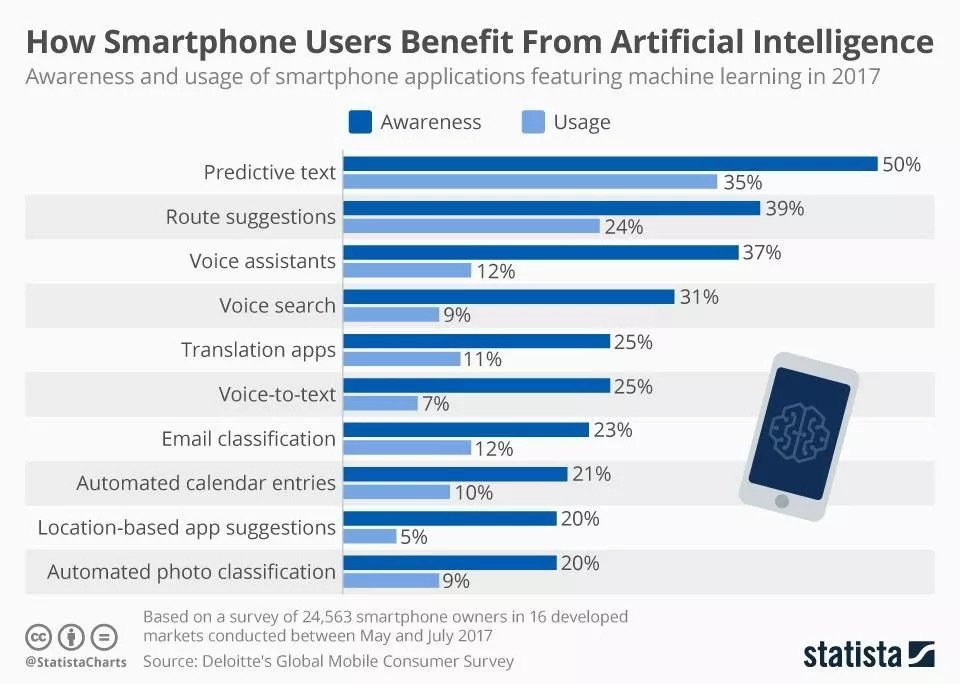
\includegraphics[width=12cm]{mobile_apps.jpg}
    \caption{Benefits from \emph{ML} to Mobile}
    \label{fig:my_label}
\end{figure}

Developing mobile applications with focus on \emph{ML} has never been easier and \emph{Google} has to take credit for it. The \emph{ML Kit} allows the developer to easily integrated \emph{machine learning} modules, made by \emph{Google}, into the application. \emph{ML Kit} can be used either on \emph{Android} and \emph{iPhone}. This tool can process data on the cloud or in the device itself.\\

Some benefits of processing the data offline are:
\begin{itemize}
    \item Increased privacy;
    \item No internet connection is required;
    \item Decreased latency, since there is no communication with the server. 
\end{itemize}

An alternative tool, which gives the developer more flexibility and control, when compared to \emph{ML Kit} would be \emph{TensorFlow Lite}, also created by \emph{Google}.

\subsection{A brave new world}
But machine learning techniques integrated in mobile applications are only a part of what this cooperation has given to the world. One of its most recent results was the Internet of Things (\emph{IoT}).\\

\emph{IoT} existed without machine learning, in fact, you could define it by simply put a group of objects with embedded sensors and software that could talk to each other. However, just like with smartphones, when you had machine learning to the equation everything seems more interesting.\\

A good example of it is \emph{Google}'s \emph{Nest Thermostat}, this thermostat uses machine learning to predict the ideal the correct temperature for the house when you return home from work or when you get up in the morning.
\section{Future perspective}
Both these technologies will keep growing in the future. machine learning has given us in the last few years a tailored customer experience that many of us cannot imagine leaving without. The increasing adoption of \emph{IoT} and our dependency on our smartphones has shown us that the way we interact with technology has changed and, probably, will keep changing towards a more fluid experience.

\printbibliography


\end{document}